\documentclass[oneside,a4paper]{amsart}
%\usepackage{maa-monthly}
\usepackage{gauss-bonnet}
%\usepackage[russian,english]{babel}
%\usepackage[utf8]{inputenc}

\begin{document}

\title{Self-crossings of closed geodesics}
\author{Anton Petrunin and Sergio Zamora Barrera}
%\address{Anton Petrunin,  Math. Dept., PSU, University Park,  PA 16802, USA.}
%\address{aqp6@psu.edu}
%\address{Sergio Zamora Barrera,  Math. Dept., PSU,University Park,  PA 16802, USA.}
%\address{sxz38@psu.edu}

%\keywords{discrete minimal surface, polyhedral surface, area minimizing surface, minimal surface.}
\maketitle

\section{Introduction}


The rubber bend on the picture is pulled around a pebble,
and it crosses it-self at several points.
\begin{figure}[!ht]
\begin{minipage}{.64\textwidth}
\centering
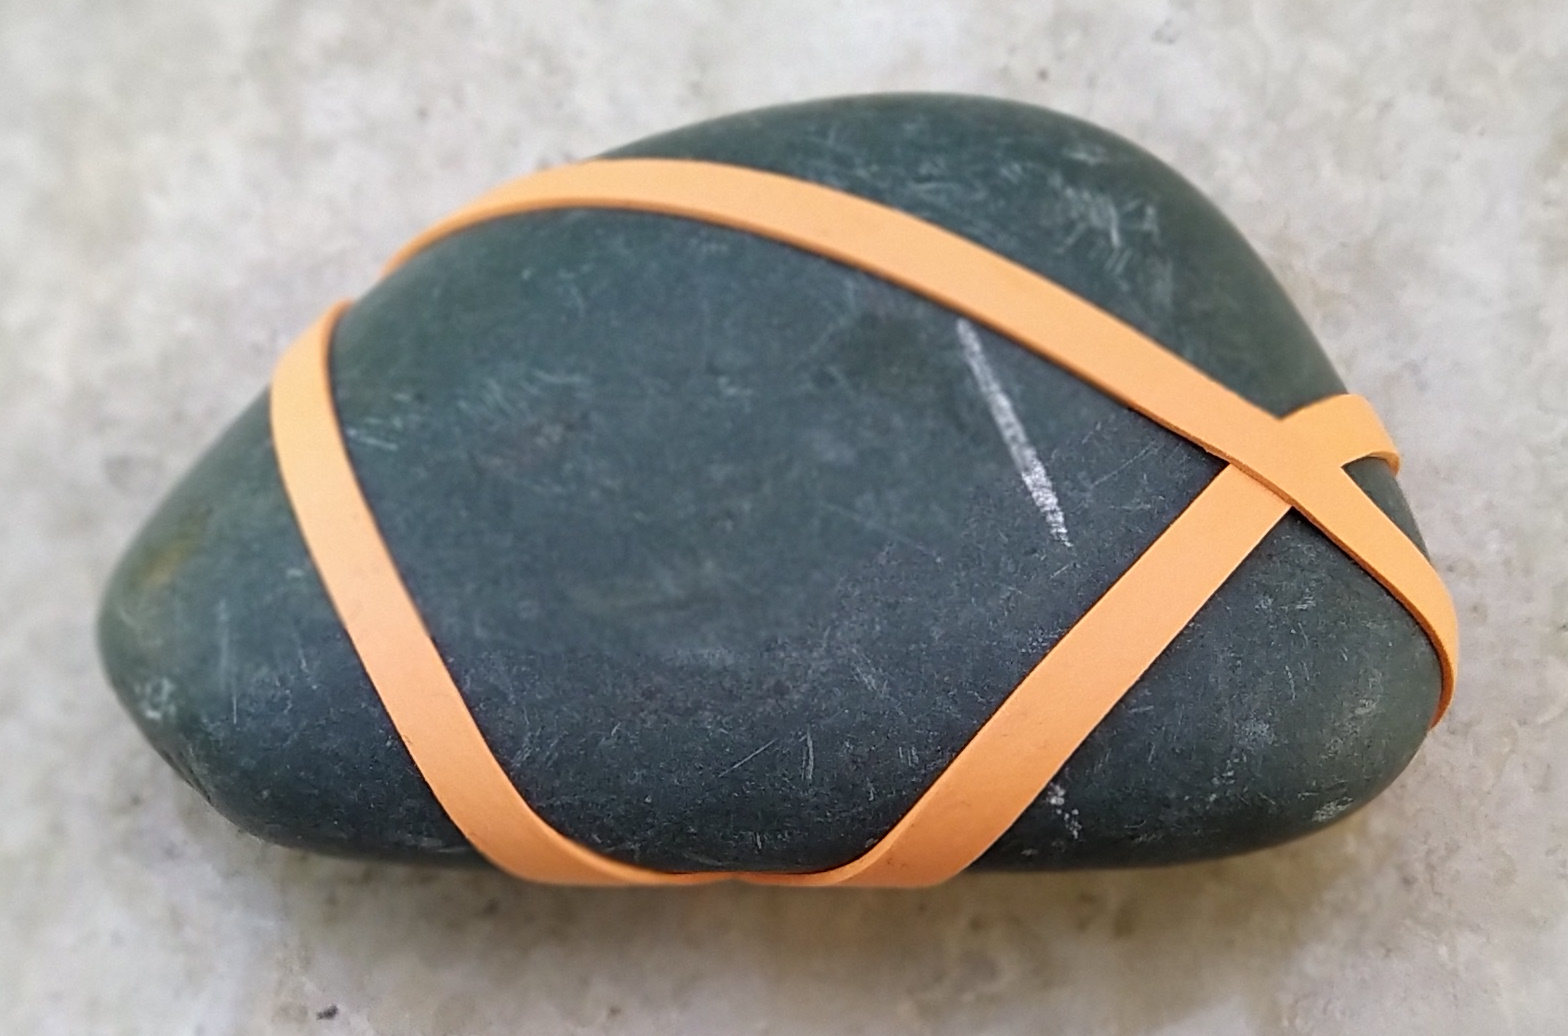
\includegraphics[width=\textwidth]{pics/pebble.jpg}
\end{minipage}\hfill
\begin{minipage}{.34\textwidth}
\centering
\includegraphics{mppics/pic-50}
\end{minipage}
\end{figure}
The combinatorics of self-crossings can be described by  closed plane curve.
To do this, look at the curve that rubber band follow in a plane parametrization of the surface with one point removed.
For example, the self-crossings of rubber band on the picture can be described by the plane curves on the right diagram;
one has to turn it around to see it.

\begin{thm}{Problem} What are the possible combinatoric types of self-crossings of rubber band for all possible pebbles; we assume that the pebble is strictly convex and its surface is smooth
and frictionless.
\end{thm}

For sure the rubber band should be understood as closed geodesic on smooth strictly convex surface.

This problem is exotic, but it makes a good exercise.
One one hand, it could be explained informally to anyone.
On the other hand, if a motivated student starts to think about this problem on an isolated island, then he will have to rediscover  a considerable part of the differential geometry of surfaces.
Or, one could use this problem to measure progress while taking an introductory course of differential geometry.

As you will see, configurations with at most 3 double self-crossings is already interesting;
the solutions are short, but require creativity.

The following diagram shows all possible paterns with exactly 3 double self-crossings.
\begin{figure}[ht!]
\begin{center}
\includegraphics{mppics/pic-55}
\end{center}
\end{figure}
All except the last two can be realized by a closed geodesic on a smooth strictly convex closed surface.

Construction of some of these examples require ingenuity,
but, the forbidden examples make mathematicians way more happier.
(It is strange that mathematicians like to forbid, is not it?)

In this note we will discuss the two forbidden examples --- fifth and sixth.
The proofs require Gauss--Bonnet formula and Alexandrov comparison theorem respectively.
Both of these statements are briefly discussed in the following sectio.

\section*{Comparison theorems}

Further we assume that $\Sigma$ is a closed strictly convex surface;
in particular, $\Sigma$ is homeomorphic to the sphere and has strictly positive Gauss curvature.

Suppose that $\Delta$ is an $n$-gon on $\Sigma$ with geodesic sides.
From the \emph{Gauss--Bonnet formula} it follows that sum of the internal angles of $\Delta$ cannot be smaller than $(n\z-2)\cdot\pi$.
Also the Gauss--Bonnet formula implies that the integral of Gauss curvature along the whole $\Sigma$ is exactly $4\cdot\pi$.

In particular, if $\Delta$ is a triangle with angles $\alpha$, $\beta$, and $\gamma$, then
\[\alpha+\beta+\gamma>\pi.\leqno({*})\]

If we assume in addition that the sides of $\Delta$ are length minimizing geodesics among the curves in $\Delta$ with the same endpoints, then the inequality $({*})$ can be made more exact.

Namely consider the so-called \emph{model triangle} $\tilde\Delta$ of $\Delta$; that is, $\tilde\Delta$ is a plane triangle with equal corresponding sides.
Since the sides are length-minimizing in $\Delta$, they satisfy the triangle inequality; therefore the model triangle is defined.

Denote bu $\tilde \alpha$, $\tilde \beta$ and $\tilde \gamma$ the angles of $\tilde\Delta$ respectively.
Then 
\[
\alpha> \tilde \alpha,
\qquad
\beta> \tilde \beta,
\qquad
\text{and}
\qquad
\gamma> \tilde \gamma.
\leqno({*}{*})
\]
Since $\tilde\alpha+\tilde\beta+\tilde\gamma=\pi$, this inequality implies $({*})$.

The inequality $({*}{*})$ easily follows from the proof of the \emph{Alexandrov--Toponogov comparison theorem}.
We leave it as an exercise to those who knows this proof;
the rest of the readers should simply believe that it is true.

\section*{Fifth configuration}

\begin{wrapfigure}{r}{40 mm}
\vskip-0mm
\centering
\includegraphics{mppics/pic-3}
\end{wrapfigure}

Let us show that the fifth configuration is impossible.
Suppose there is a geodesic of with self-crossings as on the diagram;
it divides the surface $\Sigma$ into one triangle, say $\Delta$, one hexagon and three monogons.
Denote by $\alpha$, $\beta$, and $\gamma$ the internal angles of $\Delta$.

Note that three monogons have internal angles $\alpha$, $\beta$, and $\gamma$ respectively.
By Gauss--Bonnet formula, the integral of Gauss curvature along each monogon is $\pi+\alpha$, $\pi+\beta$, and $\pi+\gamma$ respectively.
By $({*})$ the integral of Gauss curvature along the whole $\Sigma$ exceeds $4\cdot \pi$ --- a contradiction.

\section*{Sixth configuration}

Arguing by contradiction, suppose that $\Sigma$ contains such a geodesic $\gamma$;
assume that arcs and angles are labeled as on the left diagram.

\begin{figure}[!ht]
\begin{minipage}{.38\textwidth}
\centering
\includegraphics{mppics/pic-472}
\end{minipage}\hfill
\begin{minipage}{.58\textwidth}
\centering
\includegraphics{mppics/pic-473}
\end{minipage}
\end{figure}


Applying the Gauss--Bonnet formula to the quadrangle and pentagon that the geodesic cuts from $\Sigma$, we get that
\[2\cdot\alpha<\beta+\gamma
\qquad\text{and} \qquad
2\cdot\beta+2\cdot \gamma<\pi+\alpha.\leqno(\asterism)\]
It follows that $\alpha <\tfrac \pi 3$.


Consider the part of $\gamma$ without the arc~$a$.
It cuts from $\Sigma$ a pentagon $\Delta$ with sides and angles shown on the diagram on the right.

\begin{wrapfigure}{r}{50 mm}
\vskip-0mm
\centering
\includegraphics{mppics/pic-474}
\bigskip
\includegraphics{mppics/pic-500}
\vskip8mm
\end{wrapfigure}

Let us add additional vertices of the sides of $\Delta$ so that each side becomes length-minimizing.
Choose a vertex $v$ and subdivide $\Delta$ into triangles by joining $v$ to other vertices of the broken geodesic.

Consider a model triangle for each triangle in the subdivision so that they shared sides as in $\Delta$.
By the comparison inequality $({*}{*})$, the angles of the model triangles do not exceed the corresponding angles of the original triangle.
Therefore the model triangles form a plane polygon $\tilde\Delta$ is convex.
Moreover, the five angles of $\tilde\Delta$ that correspond to angles of $\Delta$ do not exceed those. 

It remains to show described plane polygogon does not exist.
Let us orient its  sides counterclockwise;
denote the obtained vectors by $s_1,\dots,s_k$.

On the other hand, the conditions on the angles of polygons imply that the vectors $s_i$ point in the complement of white sectors shown with angles marked on the diagram.
The sum of magnitudes of the vectors in each black sector is also marked.
Let $v$, $v'$, $w$, $w'$ be the marked unit vectors;
set $r=v+v'+w+w'$.
Observe that $(\asterism)$ implies that $r\ne 0$,
and, moreover, 
\[\langle r,s_1\rangle+\dots+\langle r,s_k\rangle>0,\]
but  $s_1+\dots+s_k=0$ --- a contradiction.




{\sloppy
\printbibliography[heading=bibintoc]
\fussy
}

\end{document}
